\documentclass[]{article}
\usepackage{lmodern}
\usepackage{amssymb,amsmath}
\usepackage{ifxetex,ifluatex}
\usepackage{fixltx2e} % provides \textsubscript
\ifnum 0\ifxetex 1\fi\ifluatex 1\fi=0 % if pdftex
  \usepackage[T1]{fontenc}
  \usepackage[utf8]{inputenc}
\else % if luatex or xelatex
  \ifxetex
    \usepackage{mathspec}
  \else
    \usepackage{fontspec}
  \fi
  \defaultfontfeatures{Ligatures=TeX,Scale=MatchLowercase}
\fi
% use upquote if available, for straight quotes in verbatim environments
\IfFileExists{upquote.sty}{\usepackage{upquote}}{}
% use microtype if available
\IfFileExists{microtype.sty}{%
\usepackage{microtype}
\UseMicrotypeSet[protrusion]{basicmath} % disable protrusion for tt fonts
}{}
\usepackage[margin=2.54cm]{geometry}
\usepackage{hyperref}
\hypersetup{unicode=true,
            pdftitle={Assignment: Spatial Analysis in R},
            pdfauthor={Sebastian Bognar},
            pdfborder={0 0 0},
            breaklinks=true}
\urlstyle{same}  % don't use monospace font for urls
\usepackage{color}
\usepackage{fancyvrb}
\newcommand{\VerbBar}{|}
\newcommand{\VERB}{\Verb[commandchars=\\\{\}]}
\DefineVerbatimEnvironment{Highlighting}{Verbatim}{commandchars=\\\{\}}
% Add ',fontsize=\small' for more characters per line
\usepackage{framed}
\definecolor{shadecolor}{RGB}{248,248,248}
\newenvironment{Shaded}{\begin{snugshade}}{\end{snugshade}}
\newcommand{\KeywordTok}[1]{\textcolor[rgb]{0.13,0.29,0.53}{\textbf{#1}}}
\newcommand{\DataTypeTok}[1]{\textcolor[rgb]{0.13,0.29,0.53}{#1}}
\newcommand{\DecValTok}[1]{\textcolor[rgb]{0.00,0.00,0.81}{#1}}
\newcommand{\BaseNTok}[1]{\textcolor[rgb]{0.00,0.00,0.81}{#1}}
\newcommand{\FloatTok}[1]{\textcolor[rgb]{0.00,0.00,0.81}{#1}}
\newcommand{\ConstantTok}[1]{\textcolor[rgb]{0.00,0.00,0.00}{#1}}
\newcommand{\CharTok}[1]{\textcolor[rgb]{0.31,0.60,0.02}{#1}}
\newcommand{\SpecialCharTok}[1]{\textcolor[rgb]{0.00,0.00,0.00}{#1}}
\newcommand{\StringTok}[1]{\textcolor[rgb]{0.31,0.60,0.02}{#1}}
\newcommand{\VerbatimStringTok}[1]{\textcolor[rgb]{0.31,0.60,0.02}{#1}}
\newcommand{\SpecialStringTok}[1]{\textcolor[rgb]{0.31,0.60,0.02}{#1}}
\newcommand{\ImportTok}[1]{#1}
\newcommand{\CommentTok}[1]{\textcolor[rgb]{0.56,0.35,0.01}{\textit{#1}}}
\newcommand{\DocumentationTok}[1]{\textcolor[rgb]{0.56,0.35,0.01}{\textbf{\textit{#1}}}}
\newcommand{\AnnotationTok}[1]{\textcolor[rgb]{0.56,0.35,0.01}{\textbf{\textit{#1}}}}
\newcommand{\CommentVarTok}[1]{\textcolor[rgb]{0.56,0.35,0.01}{\textbf{\textit{#1}}}}
\newcommand{\OtherTok}[1]{\textcolor[rgb]{0.56,0.35,0.01}{#1}}
\newcommand{\FunctionTok}[1]{\textcolor[rgb]{0.00,0.00,0.00}{#1}}
\newcommand{\VariableTok}[1]{\textcolor[rgb]{0.00,0.00,0.00}{#1}}
\newcommand{\ControlFlowTok}[1]{\textcolor[rgb]{0.13,0.29,0.53}{\textbf{#1}}}
\newcommand{\OperatorTok}[1]{\textcolor[rgb]{0.81,0.36,0.00}{\textbf{#1}}}
\newcommand{\BuiltInTok}[1]{#1}
\newcommand{\ExtensionTok}[1]{#1}
\newcommand{\PreprocessorTok}[1]{\textcolor[rgb]{0.56,0.35,0.01}{\textit{#1}}}
\newcommand{\AttributeTok}[1]{\textcolor[rgb]{0.77,0.63,0.00}{#1}}
\newcommand{\RegionMarkerTok}[1]{#1}
\newcommand{\InformationTok}[1]{\textcolor[rgb]{0.56,0.35,0.01}{\textbf{\textit{#1}}}}
\newcommand{\WarningTok}[1]{\textcolor[rgb]{0.56,0.35,0.01}{\textbf{\textit{#1}}}}
\newcommand{\AlertTok}[1]{\textcolor[rgb]{0.94,0.16,0.16}{#1}}
\newcommand{\ErrorTok}[1]{\textcolor[rgb]{0.64,0.00,0.00}{\textbf{#1}}}
\newcommand{\NormalTok}[1]{#1}
\usepackage{graphicx,grffile}
\makeatletter
\def\maxwidth{\ifdim\Gin@nat@width>\linewidth\linewidth\else\Gin@nat@width\fi}
\def\maxheight{\ifdim\Gin@nat@height>\textheight\textheight\else\Gin@nat@height\fi}
\makeatother
% Scale images if necessary, so that they will not overflow the page
% margins by default, and it is still possible to overwrite the defaults
% using explicit options in \includegraphics[width, height, ...]{}
\setkeys{Gin}{width=\maxwidth,height=\maxheight,keepaspectratio}
\IfFileExists{parskip.sty}{%
\usepackage{parskip}
}{% else
\setlength{\parindent}{0pt}
\setlength{\parskip}{6pt plus 2pt minus 1pt}
}
\setlength{\emergencystretch}{3em}  % prevent overfull lines
\providecommand{\tightlist}{%
  \setlength{\itemsep}{0pt}\setlength{\parskip}{0pt}}
\setcounter{secnumdepth}{0}
% Redefines (sub)paragraphs to behave more like sections
\ifx\paragraph\undefined\else
\let\oldparagraph\paragraph
\renewcommand{\paragraph}[1]{\oldparagraph{#1}\mbox{}}
\fi
\ifx\subparagraph\undefined\else
\let\oldsubparagraph\subparagraph
\renewcommand{\subparagraph}[1]{\oldsubparagraph{#1}\mbox{}}
\fi

%%% Use protect on footnotes to avoid problems with footnotes in titles
\let\rmarkdownfootnote\footnote%
\def\footnote{\protect\rmarkdownfootnote}

%%% Change title format to be more compact
\usepackage{titling}

% Create subtitle command for use in maketitle
\providecommand{\subtitle}[1]{
  \posttitle{
    \begin{center}\large#1\end{center}
    }
}

\setlength{\droptitle}{-2em}

  \title{Assignment: Spatial Analysis in R}
    \pretitle{\vspace{\droptitle}\centering\huge}
  \posttitle{\par}
    \author{Sebastian Bognar}
    \preauthor{\centering\large\emph}
  \postauthor{\par}
    \date{}
    \predate{}\postdate{}
  

\begin{document}
\maketitle

{
\setcounter{tocdepth}{2}
\tableofcontents
}
\subsection{OVERVIEW}\label{overview}

This exercise accompanies the lessons in Environmental Data Analytics
(ENV872L) on spatial analysis.

\subsection{Directions}\label{directions}

\begin{enumerate}
\def\labelenumi{\arabic{enumi}.}
\tightlist
\item
  Change ``Student Name'' on line 3 (above) with your name.
\item
  Use the lesson as a guide. It contains code that can be modified to
  complete the assignment.
\item
  Work through the steps, \textbf{creating code and output} that fulfill
  each instruction.
\item
  Be sure to \textbf{answer the questions} in this assignment document.
  Space for your answers is provided in this document and is indicated
  by the ``\textgreater{}'' character. If you need a second paragraph be
  sure to start the first line with ``\textgreater{}''. You should
  notice that the answer is highlighted in green by RStudio.
\item
  When you have completed the assignment, \textbf{Knit} the text and
  code into a single HTML file.
\item
  After Knitting, please submit the completed exercise (HTML file) to
  the dropbox in Sakai. Please add your last name into the file name
  (e.g., ``Fay\_A09\_SpatialAnalysis.pdf'') prior to submission.
\end{enumerate}

\subsection{DATA WRANGLING}\label{data-wrangling}

\subsubsection{1. Prepare the workspace}\label{prepare-the-workspace}

\begin{itemize}
\tightlist
\item
  Import: tidyverse, sf, and leaflet
\end{itemize}

\begin{Shaded}
\begin{Highlighting}[]
\CommentTok{# import tidyverse, sf, and leaflet}
\KeywordTok{library}\NormalTok{(tidyverse)}
\end{Highlighting}
\end{Shaded}

\begin{verbatim}
## -- Attaching packages ----------------------------------------------------------------------------- tidyverse 1.2.1 --
\end{verbatim}

\begin{verbatim}
## v ggplot2 3.1.0       v purrr   0.3.2  
## v tibble  2.1.1       v dplyr   0.8.0.1
## v tidyr   0.8.3       v stringr 1.4.0  
## v readr   1.3.1       v forcats 0.4.0
\end{verbatim}

\begin{verbatim}
## -- Conflicts -------------------------------------------------------------------------------- tidyverse_conflicts() --
## x dplyr::filter() masks stats::filter()
## x dplyr::lag()    masks stats::lag()
\end{verbatim}

\begin{Shaded}
\begin{Highlighting}[]
\KeywordTok{library}\NormalTok{(sf)}
\end{Highlighting}
\end{Shaded}

\begin{verbatim}
## Linking to GEOS 3.6.1, GDAL 2.1.3, PROJ 4.9.3
\end{verbatim}

\begin{Shaded}
\begin{Highlighting}[]
\KeywordTok{library}\NormalTok{(leaflet)}
\KeywordTok{library}\NormalTok{(mapview)}
\KeywordTok{library}\NormalTok{(ggplot2)}
\end{Highlighting}
\end{Shaded}

\subsubsection{2. Read filtered county features into an sf dataframe and
plot}\label{read-filtered-county-features-into-an-sf-dataframe-and-plot}

In this exercise, we will be exploring stream gage height data in
Nebraska, as there's been recent floods there. First, we will import
from the US Counties\\
shapefile we've used in lab lessons, filtering it this time for just
Nebraska counties. Nebraska's state FIPS code is \texttt{31} (as North
Carolina's was \texttt{37}).

\begin{itemize}
\tightlist
\item
  Read the cb\_2017\_us\_county\_20m.shp shapefile into an sf dataframe
\item
  Filter for Nebraska counties (State FIPS = 31)
\item
  Show the dataset's coordinate reference system
\item
  Plot the records as a map (in any format)
\end{itemize}

\begin{Shaded}
\begin{Highlighting}[]
\CommentTok{#Read in Counties shapefile into an sf dataframe, filtering for just NC counties}
\NormalTok{counties<-}\StringTok{ }\KeywordTok{st_read}\NormalTok{(}\StringTok{'./Data/Spatial/cb_2017_us_county_20m.shp'}\NormalTok{) }\OperatorTok
\StringTok{  }\KeywordTok{filter}\NormalTok{(STATEFP }\OperatorTok{==}\StringTok{ }\DecValTok{31}\NormalTok{)}
\end{Highlighting}
\end{Shaded}

\begin{verbatim}
## Reading layer `cb_2017_us_county_20m' from data source `/Users/Seabass/Documents/Duke/spring_2019/env_872L/lesson_2/ENV_872L/Data/Spatial/cb_2017_us_county_20m.shp' using driver `ESRI Shapefile'
## Simple feature collection with 3220 features and 9 fields
## geometry type:  MULTIPOLYGON
## dimension:      XY
## bbox:           xmin: -179.1743 ymin: 17.91377 xmax: 179.7739 ymax: 71.35256
## epsg (SRID):    4269
## proj4string:    +proj=longlat +datum=NAD83 +no_defs
\end{verbatim}

\begin{Shaded}
\begin{Highlighting}[]
\CommentTok{#Reveal the CRS of the counties features}
\KeywordTok{st_crs}\NormalTok{(counties)}
\end{Highlighting}
\end{Shaded}

\begin{verbatim}
## Coordinate Reference System:
##   EPSG: 4269 
##   proj4string: "+proj=longlat +datum=NAD83 +no_defs"
\end{verbatim}

\begin{Shaded}
\begin{Highlighting}[]
\CommentTok{#Plot the data}
\KeywordTok{plot}\NormalTok{(counties[}\StringTok{'COUNTYNS'}\NormalTok{])}
\end{Highlighting}
\end{Shaded}

\includegraphics{Bognar_A09_SpatialAnalysis_files/figure-latex/Read the county data into an sf dataframe-1.pdf}
\textgreater{} QUESTION: What is the EPSG code of the Counties dataset?
Using \url{http://spatialreference.org}, is this a geographic or a
projected coordinate system? (Or, does this CRS use angular or planar
coordinate units?) To what datum is this CRS associated?\\
\textgreater{} ANSWER: The EPSG code of the Counties dataset is 4269 and
it is a geographic coordinate system. The CRS uses angular coordinate
units. The data that the CRS is associated with is NAD83.

\subsubsection{3. Read in gage locations csv as a dataframe, then
display the column names it
contains}\label{read-in-gage-locations-csv-as-a-dataframe-then-display-the-column-names-it-contains}

Next we'll read in some USGS/NWIS gage location data I've added to the
\texttt{Data/Raw} folder. These are in the
\texttt{NWIS\_SiteInfo\_NE\_RAW.csv} file. (See
\texttt{NWIS\_SiteInfo\_NE\_RAW.README.txt} for more info on this
datset.) * Read the NWIS\_SiteInfo\_NE\_RAW.csv file into a standard
dataframe * Display the column names of this dataset

\begin{Shaded}
\begin{Highlighting}[]
\CommentTok{#Read in gage locations csv as a dataframe}
\NormalTok{NWIS_RAW <-}\StringTok{ }\KeywordTok{read.csv}\NormalTok{(}\StringTok{"./Data/Raw/NWIS_SiteInfo_NE_RAW.csv"}\NormalTok{)}

\CommentTok{#Reveal the names of the columns}
\KeywordTok{colnames}\NormalTok{(NWIS_RAW)}
\end{Highlighting}
\end{Shaded}

\begin{verbatim}
## [1] "site_no"            "station_nm"         "site_tp_cd"        
## [4] "dec_lat_va"         "dec_long_va"        "coord_acy_cd"      
## [7] "dec_coord_datum_cd"
\end{verbatim}

\begin{quote}
QUESTION: What columns in the dataset contain the x and y coordinate
values, respectively? ANSWER: ``dec\_lat\_va'' (latitude) contain the y
coordinate and the ``dec\_long\_va'' (longitude) contain the x
coordinate.
\end{quote}

\subsubsection{4. Convert the gage locations dataframe to an sf
dataframe of
points}\label{convert-the-gage-locations-dataframe-to-an-sf-dataframe-of-points}

\begin{itemize}
\tightlist
\item
  This data use the same coordnate reference system as the counties
  dataset
\item
  Display the column names of the resulting sf dataframe
\end{itemize}

\begin{Shaded}
\begin{Highlighting}[]
\CommentTok{#Convert to an sf object}

\NormalTok{NWIS_GAGE_SF <-}\StringTok{ }\KeywordTok{st_as_sf}\NormalTok{(NWIS_RAW,}\DataTypeTok{coords =} \KeywordTok{c}\NormalTok{(}\StringTok{'dec_long_va'}\NormalTok{,}\StringTok{'dec_lat_va'}\NormalTok{),}\DataTypeTok{crs=}\DecValTok{4269}\NormalTok{)}

\CommentTok{#Reveal the structure}

\KeywordTok{colnames}\NormalTok{(NWIS_GAGE_SF)}
\end{Highlighting}
\end{Shaded}

\begin{verbatim}
## [1] "site_no"            "station_nm"         "site_tp_cd"        
## [4] "coord_acy_cd"       "dec_coord_datum_cd" "geometry"
\end{verbatim}

\begin{quote}
QUESTION: What new field(s) appear in the sf dataframe created? What
field(s), if any, disappeared? ANSWER: The new field that appears is
``geometry''. ``dec\_lat\_va'' and ``dec\_long\_va'' fields disappeared.
\end{quote}

\subsubsection{\texorpdfstring{5. Use \texttt{ggplot} to plot the gage
locations on top of the
counties}{5. Use ggplot to plot the gage locations on top of the counties}}\label{use-ggplot-to-plot-the-gage-locations-on-top-of-the-counties}

\begin{itemize}
\tightlist
\item
  Plot the different datasets in different colors
\end{itemize}

\begin{Shaded}
\begin{Highlighting}[]
\KeywordTok{ggplot}\NormalTok{() }\OperatorTok{+}\StringTok{ }
\StringTok{  }\KeywordTok{geom_sf}\NormalTok{(}\DataTypeTok{data =}\NormalTok{ counties,}\DataTypeTok{col=}\StringTok{'black'}\NormalTok{) }\OperatorTok{+}\StringTok{ }
\StringTok{  }\KeywordTok{geom_sf}\NormalTok{(}\DataTypeTok{data =}\NormalTok{ NWIS_GAGE_SF,}\DataTypeTok{col=}\StringTok{'red'}\NormalTok{)}\OperatorTok{+}
\StringTok{  }\KeywordTok{ggtitle}\NormalTok{(}\StringTok{"Gage locations in the Counties of Nebraska"}\NormalTok{)}
\end{Highlighting}
\end{Shaded}

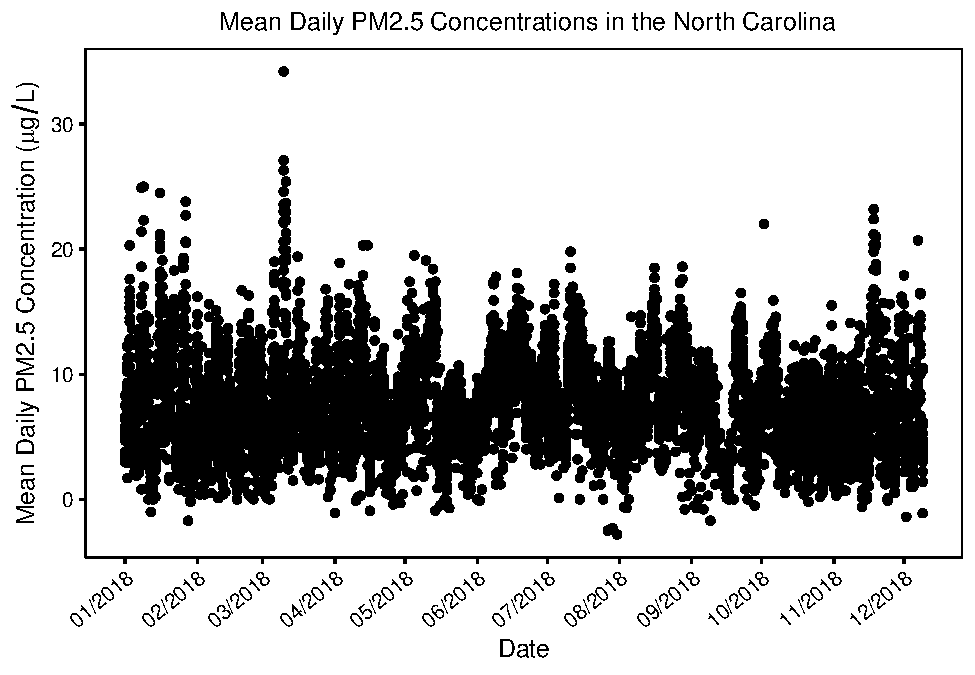
\includegraphics{Bognar_A09_SpatialAnalysis_files/figure-latex/unnamed-chunk-2-1.pdf}

\subsubsection{6. Read in the gage height data and join the site
location data to
it.}\label{read-in-the-gage-height-data-and-join-the-site-location-data-to-it.}

And finally, we want to attach some gage height data to our site
locations. I've constructed a csv file listing many of the Nebraska gage
sites, by station name and site number along with stream gage heights
(in meters) recorded during the recent flood event. This file is titled
\texttt{NWIS\_SiteFlowData\_NE\_RAW.csv} and is found in the Data/Raw
folder.

\begin{itemize}
\tightlist
\item
  Read this dataset in as a dataframe.
\item
  Join our site information (already imported above) to these gage
  height data.
\item
  The \texttt{site\_no} and \texttt{station\_nm} can both serve as
  joining attributes.
\item
  Construct this join so that the result only includes records where
  both tables have data.
\item
  Show the column names in this resulting dataframe
\item
  Once joined, we will again have to convert this product (a dataframe)
  into a spatial dataframe. Do that.
\end{itemize}

\begin{Shaded}
\begin{Highlighting}[]
\CommentTok{#Read in the data}

\NormalTok{GAGE_HEIGHT_DATA_RAW <-}\StringTok{ }\KeywordTok{read.csv}\NormalTok{(}\StringTok{"./Data/Raw/NWIS_SiteFlowData_NE_RAW.csv"}\NormalTok{)}

\CommentTok{#Show the column names}

\KeywordTok{colnames}\NormalTok{(GAGE_HEIGHT_DATA_RAW)}
\end{Highlighting}
\end{Shaded}

\begin{verbatim}
## [1] "site_no"    "station_nm" "date"       "gage_ht"
\end{verbatim}

\begin{Shaded}
\begin{Highlighting}[]
\CommentTok{#Join location data to it}

\NormalTok{GAGE_HEIGHT_SF_JOIN<-}\KeywordTok{drop_na}\NormalTok{(}\KeywordTok{left_join}\NormalTok{(NWIS_GAGE_SF,GAGE_HEIGHT_DATA_RAW, }\DataTypeTok{by =} \StringTok{"site_no"}\NormalTok{ ))}

\CommentTok{#colnames of join dataframe}

\KeywordTok{colnames}\NormalTok{(GAGE_HEIGHT_SF_JOIN)}
\end{Highlighting}
\end{Shaded}

\begin{verbatim}
## [1] "site_no"            "station_nm.x"       "site_tp_cd"        
## [4] "coord_acy_cd"       "dec_coord_datum_cd" "station_nm.y"      
## [7] "date"               "gage_ht"            "geometry"
\end{verbatim}

\begin{Shaded}
\begin{Highlighting}[]
\CommentTok{#Convert back to sf dataframe}
\NormalTok{GAGE_HEIGHT_SF <-}\StringTok{ }\KeywordTok{st_as_sf}\NormalTok{(GAGE_HEIGHT_SF_JOIN, }\DataTypeTok{coords =} \StringTok{"geometry"}\NormalTok{, }\DataTypeTok{crs=}\DecValTok{4269}\NormalTok{ )}
\end{Highlighting}
\end{Shaded}

\subsubsection{7. Map the pattern of gage height
data}\label{map-the-pattern-of-gage-height-data}

Now we can examine where the flooding appears most acute by visualizing
gage heights spatially. * Plot the gage sites on top of counties * Show
the magnitude of gage height by color, shape, other visualization
technique.

\begin{Shaded}
\begin{Highlighting}[]
\CommentTok{#Plot the values}
\KeywordTok{ggplot}\NormalTok{() }\OperatorTok{+}\StringTok{ }
\StringTok{  }\KeywordTok{geom_sf}\NormalTok{(}\DataTypeTok{data=}\NormalTok{counties, }\DataTypeTok{fill =}\StringTok{"grey"}\NormalTok{)}\OperatorTok{+}
\StringTok{  }\KeywordTok{geom_sf}\NormalTok{(}\DataTypeTok{data=}\NormalTok{GAGE_HEIGHT_SF, }\KeywordTok{aes}\NormalTok{(}\DataTypeTok{color=}\NormalTok{gage_ht)) }\OperatorTok{+}
\StringTok{ }\KeywordTok{scale_color_distiller}\NormalTok{(}\StringTok{"Gage Height (m)"}\NormalTok{, }\DataTypeTok{palette =} \StringTok{"Blues"}\NormalTok{, }\DataTypeTok{direction =} \OperatorTok{-}\DecValTok{1}\NormalTok{)}\OperatorTok{+}
\StringTok{  }\KeywordTok{ggtitle}\NormalTok{(}\StringTok{"Variability of Gage Height at Gage Locations in Nebraska"}\NormalTok{)}
\end{Highlighting}
\end{Shaded}

\includegraphics{Bognar_A09_SpatialAnalysis_files/figure-latex/unnamed-chunk-4-1.pdf}

\subsection{SPATIAL ANALYSIS}\label{spatial-analysis}

Up next we will do some spatial analysis with our data. To prepare for
this, we should transform our data into a projected coordinate system.
We'll choose UTM Zone 14N (EPGS = 32614).

\subsubsection{8. Transform the counties and gage site datasets to UTM
Zone
14N}\label{transform-the-counties-and-gage-site-datasets-to-utm-zone-14n}

\begin{itemize}
\tightlist
\item
  Transform each dataset to crs 32614
\item
  Using ggplot, plot the data so that each can be seen as different
  colors
\end{itemize}

\begin{Shaded}
\begin{Highlighting}[]
\CommentTok{#Transform the counties and gage location datasets to UTM Zone 14}
\NormalTok{counties_sf_utm <-}\StringTok{ }\KeywordTok{st_transform}\NormalTok{(counties, }\DataTypeTok{c=}\DecValTok{32614}\NormalTok{)}
\NormalTok{GAGE_HEIGHT_UTM <-}\StringTok{  }\KeywordTok{st_transform}\NormalTok{(GAGE_HEIGHT_SF, }\DataTypeTok{c=}\DecValTok{32614}\NormalTok{)}
\CommentTok{#Plot the data}
\KeywordTok{ggplot}\NormalTok{() }\OperatorTok{+}\StringTok{ }
\StringTok{  }\KeywordTok{geom_sf}\NormalTok{(}\DataTypeTok{data =}\NormalTok{ counties_sf_utm,}\KeywordTok{aes}\NormalTok{(}\DataTypeTok{fill=}\NormalTok{COUNTYNS)) }\OperatorTok{+}\StringTok{ }
\StringTok{  }\KeywordTok{guides}\NormalTok{(}\DataTypeTok{fill=}\OtherTok{FALSE}\NormalTok{)}\OperatorTok{+}
\StringTok{   }\KeywordTok{geom_sf}\NormalTok{(}\DataTypeTok{data =}\NormalTok{ GAGE_HEIGHT_UTM,}\KeywordTok{aes}\NormalTok{(}\DataTypeTok{color=}\NormalTok{gage_ht))}\OperatorTok{+}
\StringTok{   }\KeywordTok{scale_color_distiller}\NormalTok{(}\StringTok{"Gage Height (m)"}\NormalTok{, }\DataTypeTok{palette =} \StringTok{"Blues"}\NormalTok{, }\DataTypeTok{direction =} \OperatorTok{-}\DecValTok{1}\NormalTok{)}\OperatorTok{+}
\StringTok{  }\KeywordTok{ggtitle}\NormalTok{(}\StringTok{"Variability of Gage Height at Gage Locations in Nebraska"}\NormalTok{)}
\end{Highlighting}
\end{Shaded}

\includegraphics{Bognar_A09_SpatialAnalysis_files/figure-latex/unnamed-chunk-5-1.pdf}
\textgreater{} QUESTION: The shape of Nebraska should look a bit
different than the one created in Step 5? Why? \textgreater{} ANSWER:
The shape if Nebraska looks a little bit different than the one created
in step 5 because UTM is a projected coordinate system, which is planar
coordinate system. This in turn leads to stretching due to trying to
convert a circular object to a planar surface.

\subsubsection{9. Select the gages falling within a given
county}\label{select-the-gages-falling-within-a-given-county}

Now let's zoom into a particular county and examine the gages located
there. * Select Lancaster county from your county sf dataframe * Select
the gage sites falling \texttt{within} that county * Remember you'll
have to create a mask and then apply that mask * Create a plot showing:
* all Nebraska counties, * the selected county, * and the gage sites in
that county

\begin{Shaded}
\begin{Highlighting}[]
\CommentTok{#Select the county}

\NormalTok{Lancaster<-}\StringTok{ }\NormalTok{counties_sf_utm }\OperatorTok
\StringTok{  }\KeywordTok{filter}\NormalTok{(NAME }\OperatorTok{==}\StringTok{ "Lancaster"}\NormalTok{)}

\CommentTok{#Create a simple features point geometry from the point}

\NormalTok{lancaster_pt<-}\StringTok{ }\KeywordTok{st_as_sf}\NormalTok{(Lancaster, }\DataTypeTok{coords =} \StringTok{"geometry"}\NormalTok{, }\DataTypeTok{crs=}\DecValTok{32614}\NormalTok{ )}


\CommentTok{#Transform the mask to match the CRS of the counties dataset}
\NormalTok{lancaster_transformed <-}\StringTok{ }\KeywordTok{st_transform}\NormalTok{(lancaster_pt, }\DataTypeTok{crs =} \KeywordTok{st_crs}\NormalTok{(GAGE_HEIGHT_UTM))}

\CommentTok{#Create a boolean mask }
\NormalTok{resultMask <-}\StringTok{ }\KeywordTok{st_intersects}\NormalTok{(lancaster_transformed,}
\NormalTok{                            GAGE_HEIGHT_UTM,}
                            \DataTypeTok{sparse =} \OtherTok{FALSE}\NormalTok{)}

\CommentTok{#use mask to select certain county}

\NormalTok{selected_gages <-}\StringTok{ }\NormalTok{GAGE_HEIGHT_UTM[resultMask,]}




\CommentTok{#Plot}

\KeywordTok{ggplot}\NormalTok{()}\OperatorTok{+}
\StringTok{  }\KeywordTok{geom_sf}\NormalTok{(}\DataTypeTok{data =}\NormalTok{ lancaster_transformed) }\OperatorTok{+}
\StringTok{  }\KeywordTok{geom_sf}\NormalTok{(}\DataTypeTok{data =}\NormalTok{ selected_gages, }\DataTypeTok{color =} \StringTok{"magenta"}\NormalTok{, }\DataTypeTok{size =}\DecValTok{2}\NormalTok{)}\OperatorTok{+}
\KeywordTok{ggtitle}\NormalTok{(}\StringTok{"Gage Sites in the County of Lancaster, Nebraska"}\NormalTok{)}
\end{Highlighting}
\end{Shaded}

\includegraphics{Bognar_A09_SpatialAnalysis_files/figure-latex/unnamed-chunk-6-1.pdf}

\subsubsection{10. Tag each gage site with the name of the county in
which it
falls}\label{tag-each-gage-site-with-the-name-of-the-county-in-which-it-falls}

A spatial join (\texttt{st\_join}) allows us to assign the attributes of
an overlapping feature onto a another feature. We will use to assign
each gage location the attributes of the county in which it is located.
* Spatially join the county features to the gage height features *
Display the list of fields in the resulting dataset * Map the gage
locations, * Include county boundaries * Displaying each gage locations
county ``NAME'' as a different color. * Display each gage size
proportional to its ``gage\_ht'' value

\begin{Shaded}
\begin{Highlighting}[]
\CommentTok{#Join features}

\NormalTok{counties_gage_join <-}\StringTok{ }\NormalTok{GAGE_HEIGHT_UTM }\OperatorTok\StringTok{ }
\StringTok{  }\KeywordTok{st_join}\NormalTok{(}\DataTypeTok{y =}\NormalTok{ counties_sf_utm)}
  
\CommentTok{#Show column names}

\KeywordTok{colnames}\NormalTok{(counties_gage_join)}
\end{Highlighting}
\end{Shaded}

\begin{verbatim}
##  [1] "site_no"            "station_nm.x"       "site_tp_cd"        
##  [4] "coord_acy_cd"       "dec_coord_datum_cd" "station_nm.y"      
##  [7] "date"               "gage_ht"            "STATEFP"           
## [10] "COUNTYFP"           "COUNTYNS"           "AFFGEOID"          
## [13] "GEOID"              "NAME"               "LSAD"              
## [16] "ALAND"              "AWATER"             "geometry"
\end{verbatim}

\begin{Shaded}
\begin{Highlighting}[]
\CommentTok{#Plot}

\KeywordTok{ggplot}\NormalTok{()}\OperatorTok{+}
\StringTok{  }\KeywordTok{geom_sf}\NormalTok{(}\DataTypeTok{data =}\NormalTok{ counties_sf_utm) }\OperatorTok{+}
\StringTok{  }\KeywordTok{geom_sf}\NormalTok{(}\DataTypeTok{data =}\NormalTok{ counties_gage_join,}\KeywordTok{aes}\NormalTok{(}\DataTypeTok{color=}\NormalTok{NAME, }\DataTypeTok{size =}\NormalTok{ gage_ht))}\OperatorTok{+}
\StringTok{  }\KeywordTok{guides}\NormalTok{(}\DataTypeTok{size=}\OtherTok{FALSE}\NormalTok{)}\OperatorTok{+}
\StringTok{  }\KeywordTok{ggtitle}\NormalTok{(}\StringTok{"Variability in Gage Height in the State of Nebraska"}\NormalTok{)}
\end{Highlighting}
\end{Shaded}

\includegraphics{Bognar_A09_SpatialAnalysis_files/figure-latex/Spatial Join-1.pdf}

\subsubsection{11. Summarize data by
county}\label{summarize-data-by-county}

Finally, we'll summarize our gage height data by county and then display
each county by it's mean gage height. * Group the spatially joined gage
location/county dataset on the county name * Compute mean gage height *
Join (non-spatially) this result to our county sf dataframe * Prior to
joining, you'll need to drop the geometry column from the gage locations
* To do this, see the \texttt{st\_drop\_geometry} function * Plot the
counties showing mean gage heights for each county * Not all counties
will have data

\begin{Shaded}
\begin{Highlighting}[]
\CommentTok{#Group and summarize}

\CommentTok{#drop na}
\NormalTok{counties_gage_join_no_NA<-}\KeywordTok{drop_na}\NormalTok{(counties_gage_join)}

\CommentTok{#find mean of gage height}
\NormalTok{mean_gage_county<-counties_gage_join_no_NA }\OperatorTok
\StringTok{  }\KeywordTok{group_by}\NormalTok{(NAME)}\OperatorTok
\StringTok{  }\KeywordTok{summarize}\NormalTok{(}\DataTypeTok{MEAN_GAGE_HEIGHT =} \KeywordTok{mean}\NormalTok{(gage_ht))}



\CommentTok{#Convert result to a simple dataframe}
\NormalTok{mean_gage_county_simple <-}\StringTok{ }\KeywordTok{st_drop_geometry}\NormalTok{(mean_gage_county)}

\CommentTok{#Join summary to County fc}
\NormalTok{counties_summary_join <-}\StringTok{ }\NormalTok{counties_sf_utm }\OperatorTok\StringTok{ }
\StringTok{  }\KeywordTok{left_join}\NormalTok{(}\DataTypeTok{y =}\NormalTok{ mean_gage_county_simple, }\DataTypeTok{by =} \StringTok{"NAME"}\NormalTok{)}

\CommentTok{#Plot}

\KeywordTok{ggplot}\NormalTok{()}\OperatorTok{+}
\StringTok{  }\KeywordTok{geom_sf}\NormalTok{(}\DataTypeTok{data =}\NormalTok{ counties_summary_join) }\OperatorTok{+}
\StringTok{  }\KeywordTok{geom_sf}\NormalTok{(}\DataTypeTok{data =}\NormalTok{ counties_summary_join,}\KeywordTok{aes}\NormalTok{(}\DataTypeTok{fill=}\NormalTok{MEAN_GAGE_HEIGHT))}\OperatorTok{+}
\StringTok{  }\KeywordTok{scale_fill_distiller}\NormalTok{(}\StringTok{"Mean Gage Height (m)"}\NormalTok{, }\DataTypeTok{palette =} \StringTok{"Blues"}\NormalTok{, }\DataTypeTok{direction =} \OperatorTok{-}\DecValTok{1}\NormalTok{)}\OperatorTok{+}
\StringTok{  }\KeywordTok{ggtitle}\NormalTok{(}\StringTok{"Mean Gage Height for the Counties of Nebraska"}\NormalTok{)}
\end{Highlighting}
\end{Shaded}

\includegraphics{Bognar_A09_SpatialAnalysis_files/figure-latex/unnamed-chunk-7-1.pdf}


\end{document}
